\section{Appendix}\label{appendix}

    \subsection{Analytical solution}\label{analytical-solution}

     A differential equation for a linearly decaying motion can be written
as:
 
            
    
    \begin{equation}
\omega_{0}^{2} y + 2 \omega_{0} \zeta \dot{y} + \ddot{y} = 0
\label{eq:linear}
\end{equation}

    

    Which has an analytical solution \cite{undefined}:

    In the usual case of having no initial roll velocity ($\phi_0=0$) this
equation can be simlified to:
 
            
    
    \begin{equation}
\begin{aligned}
\phi = \frac{\left(\zeta \operatorname{sin}\left(\omega_{0} t \sqrt{1 - \zeta^{2}}\right) + \sqrt{1 \\ - \zeta^{2}} \operatorname{cos}\left(\omega_{0} t \sqrt{1 - \zeta^{2}}\right)\right) \phi_{0} e^{- \omega_{0} t \zeta}}{\sqrt{1 - \zeta^{2}}}
\end{aligned}
\label{eq:equation}
\end{equation}

    

    And the damping coefficient $\zeta$ is very small for ships so that
$\sqrt{1-\zeta}$ is almost 1 and the solution can be further
simplified, into something that can easily be recognized as a decaying
oscillation:
 
            
    
    \begin{equation}
\phi = \phi_{0} e^{- \omega_{0} t \zeta} \operatorname{cos}\left(\omega_{0} t\right)
\label{eq:equation}
\end{equation}

    

    \subsection{Time and frequency domain}\label{time-and-frequency-domain}

 \label{se:time_and_frequency} Ikeda's method is defined in the
frequency domain, where the damping is expressed as a function of roll
angle amplitude $\phi_a$ and roll angle frequency $\omega$. The
equivalent linear damping $B_e$ (not to confuse with eddy damping
$B_E$) is a way to convert the frequency domain damping into time
domain damping \cite{7505983/FB64RGPF}, so that time domain roll
simulations can be conducted with results from Ikeda's method. The most
general way to determine $B_e$ is to assume that the energy loss due
to damping during a half cycle of roll is the same when nonlinear and
linear dampings are used \cite{7505983/RYUBZITQ}. The $B_e$ can then
be calculated as a Fourier series expansion of the damping model, which
in the case of a cubic model yields as:
 
            
    
    \begin{equation}
B_{e} = B_{1} + \frac{8 B_{2} \omega_{0} \phi_{a}}{3 \pi} + 0.75 B_{3} \omega_{0}^{2} \phi_{a}^{2}
\label{eq:equation}
\end{equation}

    

    In the case of a quadratic model $B_3=0$ and for the linear model
$B_1$ and $B_e$ are the same thing.

    The expression above gives a relation between the frequency domain
quantities $\phi_a$, $\omega$ and the time domain quantities
$B_1$, $B_2$ and $B_3$ which can be used to obtain the latter ones
from the Ikeda's method. This can be done by calculating the damping
with Ikeda's method for a variation of frequencies and amplitudes and
then fit the above expression to this damping and obtain $B_1$,
$B_2$ and $B_3$:

\[B^{Ikeda}(\phi_a, \omega) = B_e(\phi_a, \omega)\]

In the case of a roll decay test $\phi_a$ is the only parameter being
varied. In order to verify this approach, an alternative method using
the logaritmic decrement \cite{7505983/BYNJ8CFG} to obtaining the
frequency domain quantities from time series result is also used.

This method is investigated on simulation results with a quadratic
model: $B_1 = 0.05$, $B_2 = 0.9$, $A_{44} = 1.0$, $C_1 = 5.0$.
The peak values, being the only known amplitudes from this signal, is
shown in the figure below.

    \begin{figure}[H]
        \begin{center}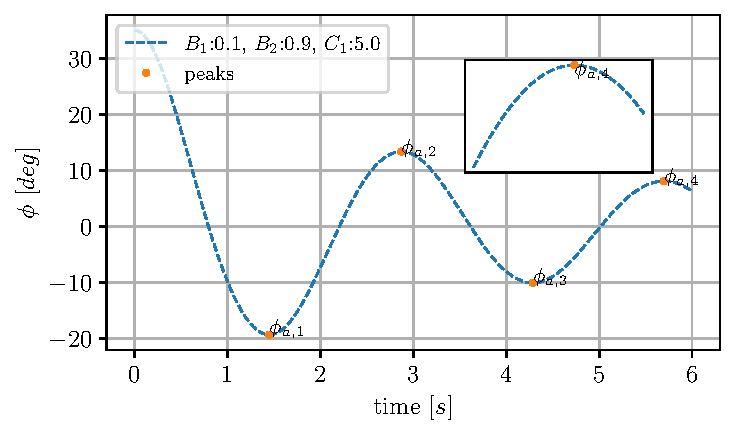
\includegraphics[width = 0.5\textwidth]{figures/peaks.pdf}\end{center}
        \vspace{-1cm}
        \caption{Peaks}
        \label{fig:peaks}
    \end{figure}
    
    The decrement is calculated as the ratio between every other peak, so
that negative and positive roll peaks are separated. This decrement can
be calulated for each peak:
\[ \Delta_n = \frac{\phi_{a,n}}{\phi_{a,n+2}}\]

    The nondimensional $\zeta$ damping coefficient for each peak can be
calculated from the logaritimic decrement:

    \[\zeta_n = \frac{\delta_n}{2\pi}=\frac{ln(\Delta_n)}{2\pi}\]

    The dimensional damping $B_n$ (Nm*s) can be then be obtained:
 
            
    
    \begin{equation}
B = 2 A_{44} \omega_{0} \zeta
\label{eq:equation}
\end{equation}

    

    So the damping can be obtained for each oscillation this way but it is
not obvious which of the roll amplitudes these dampings correspond to.
Four different choices were tried, associating damping $B_n$ with the
following amplitudes:

\begin{itemize}
\item A : $\phi_n$
\item B : $\phi_{n+1}$
\item C : $\phi_{n+2}$
\item D : $(\phi_n + \phi_{n+1} + \phi_{n+2})/3$
\end{itemize}

    \begin{figure}[H]
        \begin{center}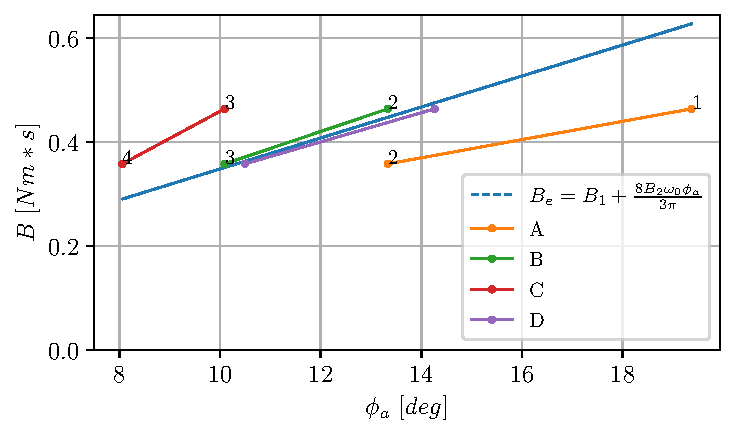
\includegraphics[width = 0.5\textwidth]{figures/logarithmic_decrement.pdf}\end{center}
        \vspace{-1cm}
        \caption{Logarithmic decrement}
        \label{fig:logarithmic_decrement}
    \end{figure}
    
    Taking the mean value of peak n and the following two peaks (alt.D) seem
to be the approach that best matches the $B_e$ (predicted using the
linearized equivalent damping method). The linearized equivalent damping
method therefore seems to be the best way to convert $B_1$, $B_2$,
$B_3$ to frequency domain, considering the difficulties with the
logaritmic decrement method as described above. The only time linearized
equivalent damping method has not been used in this paper, is when
damping at individual peaks from a time signal should be converted to
frequency domain.

    \subsection{Lewis sections}\label{lewis-sections}

    The Lewis section coefficients were calculated as:
 
            
    
    \begin{equation}
D_{1} = \frac{4 \sigma}{\pi} + \frac{\left(H_{0} - 1\right)^{2} \left(- \frac{4 \sigma}{\pi} + 1\right)}{\left(H_{0} + 1\right)^{2}} + 3
\label{eq:equation}
\end{equation}

    
 
            
    
    \begin{equation}
a_{3} = \frac{- D_{1} + \sqrt{9 - 2 D_{1}} + 3}{D_{1}}
\label{eq:equation}
\end{equation}

    
 
            
    
    \begin{equation}
a_{1} = \frac{\left(H_{0} - 1\right) \left(a_{3} + 1\right)}{H_{0} + 1}
\label{eq:equation}
\end{equation}

    

    \subsection{KVLCC2}\label{kvlcc2}
 
            
    
    
\begin{table}[H]
\small
\center
\caption{KVLCC2 section table}
\label{tab:kvlcc2_section_table}
\begin{tabular}{llllllll}
\toprule\addlinespace$x$ & $beam$ & $T_s$ & $\sigma$ & $\frac{OG}{d}$ & $R_b$ & $a_1$ & $a_3$\\ 
\midrule-0.0808 & 0.1712 & 0.0294 & 0.594 & 1.1 & 0.0976 & 0.5341 & 0.0935\\ 
0.1494 & 0.4102 & 0.2684 & 0.2433 & 0.1205 & 0.623 & -0.1824 & 0.3651\\ 
0.4125 & 0.6151 & 0.3059 & 0.4922 & 0.1058 & 0.6672 & 0.0032 & 0.1916\\ 
0.6427 & 0.7394 & 0.3059 & 0.6537 & 0.1058 & 0.6041 & 0.1024 & 0.0836\\ 
0.9058 & 0.8259 & 0.3059 & 0.7858 & 0.1058 & 0.5021 & 0.1489 & -0.0002\\ 
1.1361 & 0.851 & 0.3059 & 0.878 & 0.1058 & 0.3847 & 0.1542 & -0.0576\\ 
1.3663 & 0.8529 & 0.3059 & 0.9445 & 0.1058 & 0.2596 & 0.1482 & -0.0998\\ 
1.6294 & 0.8529 & 0.3059 & 0.9838 & 0.1058 & 0.1404 & 0.144 & -0.1255\\ 
1.8596 & 0.8529 & 0.3059 & 0.9974 & 0.1058 & 0.0566 & 0.1425 & -0.1345\\ 
2.1227 & 0.8529 & 0.3059 & 0.998 & 0.1058 & 0.0499 & 0.1424 & -0.1349\\ 
2.3529 & 0.8529 & 0.3059 & 0.998 & 0.1058 & 0.0499 & 0.1424 & -0.1349\\ 
2.5866 & 0.8529 & 0.3059 & 0.998 & 0.1058 & 0.0499 & 0.1424 & -0.1349\\ 
2.8537 & 0.8529 & 0.3059 & 0.998 & 0.1058 & 0.0499 & 0.1424 & -0.1349\\ 
3.0874 & 0.8529 & 0.3059 & 0.998 & 0.1058 & 0.0499 & 0.1424 & -0.1349\\ 
3.3211 & 0.8529 & 0.3059 & 0.9979 & 0.1058 & 0.0501 & 0.1424 & -0.1349\\ 
3.5882 & 0.8528 & 0.3059 & 0.9912 & 0.1058 & 0.1032 & 0.1431 & -0.1304\\ 
3.8219 & 0.8454 & 0.3059 & 0.9701 & 0.1058 & 0.1898 & 0.1416 & -0.1166\\ 
4.0556 & 0.8141 & 0.3059 & 0.9358 & 0.1058 & 0.273 & 0.1285 & -0.0949\\ 
4.2893 & 0.7078 & 0.3059 & 0.8981 & 0.1058 & 0.3206 & 0.0676 & -0.0718\\ 
4.5564 & 0.4148 & 0.3059 & 0.8566 & 0.1058 & 0.2911 & -0.1835 & -0.0438\\ 
4.7901 & 0.084 & 0.2379 & 0.4708 & 0.136 & 0.222 & -0.7722 & 0.103\\ 

\bottomrule
\end{tabular}
\end{table}

    

            \begin{tcolorbox}[breakable, size=fbox, boxrule=.5pt, pad at break*=1mm, opacityfill=0]
\begin{Verbatim}[commandchars=\\\{\}]
1.1223689233046326
\end{Verbatim}
\end{tcolorbox}
        
            \begin{tcolorbox}[breakable, size=fbox, boxrule=.5pt, pad at break*=1mm, opacityfill=0]
\begin{Verbatim}[commandchars=\\\{\}]
1.08
\end{Verbatim}
\end{tcolorbox}
        

    % Add a bibliography block to the postdoc
    
    
    
